%\documentclass{article}

\documentclass[9pt,twocolumn,twoside]{gsajnl}
\usepackage{amsmath}
% Use the documentclass option 'lineno' to view line numbers

\articletype{inv} % article type
% {inv} Investigation 
% {gs} Genomic Selection
% {goi} Genetics of Immunity 
% {gos} Genetics of Sex 
% {mp} Multiparental Populations

%Simulating Isolation by Distance in Continuous Space
%Space is the Place: How Dispersal and Competition Shape Genetic Variation in Continuous Space
%Impacts of Continuous Spatial Structure on Analyses of Population Genetic Data
\title{Space is the Place: How Dispersal Shapes Genetic Variation in Continuous Space}

\author[$\ast$,1]{C.J. Battey}
\author[$\dagger$,1]{Peter Ralph}
\author[$\ddagger$,2]{Andrew Kern}

\affil[$\ast$]{University of Oregon Dept. Biology, Institute for Ecology Evolution}
\keywords{Space; Population Structure; Demography; Haplotype block sharing}

\runningtitle{SPACENESS} % For use in the footer 

%% For the footnote.
%% Give the last name of the first author if only one author;
% \runningauthor{FirstAuthorLastname}
%% last names of both authors if there are two authors;
% \runningauthor{FirstAuthorLastname and SecondAuthorLastname}
%% last name of the first author followed by et al, if more than two authors.
\runningauthor{Battey \textit{et al.}}

\begin{abstract}
Individuals exist in continuous space, but standard models in population genetics are based on discrete randomly-mating populations exchanging migrants. As the availability of population-level, whole-genome data allows inference of increasingly fine-scale patterns of ancestry in many species, models incorporating realistic demographic and spatial processes are needed to accurately describe spatial structure and control for its impacts on analyses of selection and demography. Here we implement a forward-time continuous-space model of molecular evolution and use it to study the impacts of limited dispersal in continuous landscapes on population genetic summary statistics, demographic inference, and association studies. Low dispersal slows the geographic spread of ancestry and inflates branch lengths for mid-frequency alleles because of slow coalescence among distant individuals. This inflation can bias demographic inference from the site frequency spectrum towards inferring a recent spike in population sizes. In a GWAS setting spatially correlated phenotypes cause spurious signals of genetic association when principal components analyses fail to capture the relevant spatial scale of phenotypic variation, which can occur under either very limited or very high dispersal. Last we use a machine learning regression approach to evaluate summary statistics as estimators of dispersal distance and find that correlation coefficients between spatial distance and moments of the distribution of pairwise haplotype block lengths retain strong signal even at high dispersal distances. 
\end{abstract}

\begin{document}

\maketitle
\thispagestyle{firststyle}
\marginmark
\firstpagefootnote


\correspondingauthoraffiliation{3}{University of Oregon Dept. Biology, Institute for Ecology and Evolution.}
\vspace{-35pt}% Only used for adjusting extra space in the left column of the first page

\section{Introduction}
The inescapable reality that biological organisms live, move, and reproduce in continuous spatial landscapes has been all but ignored in population genetic models. 

In most sexual organisms individuals mate with other nearby individuals, leading to a positive correlation between genetic and geographic distances. This pattern of "isolation by distance" \citep{Wright1943} is one of the most widely replicated empirical findings in population genetics \citep{Chen2017,Jay2012,Sharbel2000}, but is only heuristically approximated by existing forward-time models of molecular evolution based on discrete demes exchanging migrants. As the availability of population-level whole-genome data allows inference of increasingly fine-scale patterns of ancestry in many species, models incorporating biologically realistic demographic and spatial processes are needed to accurately describe continuous spatial structure and control for its impacts on analyses of selection and demography. This situation is particularly clear in human population genetics, where individual ancestries are often interpreted as mixtures of discrete populations in part because of modeling assumptions underlying discrete clustering algorithms and association analyses are often strongly dependent on statistical corrections for population stratification \citep{Berg2018}.  

The best-studied approaches to population genetics in continuous space were developed by \citep{Wright1943} and \citep{Malecot1948}, who derived expressions for pairwise genetic differentiation in continuous space assuming Poisson distributed numbers of offspring and independent dispersal among individuals. However, \citep{Felsenstein1975} showed that these assumptions are incompatible -- over time, a population meeting them will clump into a small number of geographic clusters occupying only a part of the available range. (NOTE: where to put Rousset et al. lit?)

NOTE: probably cut this paragraph???

This process is analogous to genetic drift, with spatial locations and population densities taking the place of sites and allele frequencies. Because individuals disperse from their natal location, new offspring are likely to be close to their parents. If by chance an individual has no offspring the local population density is then lowered, which decreases the chance of new individuals dispersing into that area. This process compounds over time until only one or two patches of habitat are occupied at any given time. The resulting spatial clustering clearly does not describe spatial dynamics in most real populations, because declining growth rates in regions of high population density are common in both lab ( ) and wild populations ( ). 

One method for modeling populations in continuous space is then to assume the existence of a grid of discrete randomly-mating populations connected by migration, which prevents clustering by forcing all regions to be occupied in every generation. Though good approximations of continuous structure given high dispersal (Barton(?)), these models are not truly continuous and limit investigation of spatial structure below the level of the deme. An alternative approach is to model the geographic spread of ancestry backwards in time through a diffusion approximation -- an approach that has recently made significant progress in modeling both dispersal and demographic parameters \citep{Barton2010,Kelleher2014,Ringbauer2017,Ringbauer2018}. However, these models currently lack a well-described forward-time analog that produces biologically realistic spatial patterns. 

A direct approach to the clustering problem of classical forward-time models is to incorporate density dependence by scaling individual fitness to local population density. This shifts reproductive output towards regions of low-density, preventing populations from clustering in space over time. This approach was taken previously by \citep{Doebeli2003} who used an individual based model with continuous space and density dependent fitness to study the probability of speciation along continuous environmental gradients. (**Sentence referencing other continuous IBM's with density dependence**). However to our knowledge all previous implementations of continuous space models have focused on individuals or at most a few genotypes as the unit of analysis, which limits our ability to investigate the impacts of continuous space on genome-wide genetic variation as is now routinely sampled from real organisms. 

Here we describe an implementation of an individual-based model in continuous space that incorporates overlapping generations, a Gaussian dispersal kernel, and density-dependent fitness, and scales to chromosome-scale alignments across tens of thousands of individuals. We use this model to describe the impacts of variation in dispersal distance on a variety of summary statistics typically analyzed under discrete population models, and apply a machine-learning regression approach to evaluate a new class of summary statistics based on correlations between geographic distance and moments of the distribution of pairwise haplotype block lengths as estimators of dispersal distance. We then examine how the fine-scale spatial structures occurring under limited dispersal impact demographic inference from the site frequency spectrum; finding that inflation of branch lengths for mid-frequency alleles associated with slow coalescence of distant individuals **TBD**. 

Last, we use our model to study the impacts of isolation by distance in continuous space on genome-wide association studies (GWAS). Variation in ancestry proportions between case and control cohorts will cause inflation of test statistics at SNPs with different allele frequencies among populations (CITE). In addition, because most phenotypes are influenced by the environment and environmental factors are often spatially correlated, subtle spatial structure within and among populations can lead to inflated effect size estimates in GWAS of quantitative traits conducted on samples from large geographic regions \citep{Mathieson2012}. For example, imagine a population of flowering plants occurring over a large latitudinal range with populations subject to isolation by distance. Flowering time is strongly dependent on photoperiod and temperature, both of which typically vary with latitude. If we were to conduct a GWAS for flowering time without correcting for population structure we would find that all SNPs with allele frequencies varying clinally with latitude were significantly associated with flowering time, even if flowering time was determined purely by the environment. 

A common method of correcting for population structure in GWAS is to run a principal components analysis on the genotype matrix and include PC coordinates as covariates in a linear regression for each SNP \citep{Price2006}. Mixed model GWAS employs a different statistical framework but takes a similar approach by incorporating a kinship matrix describing pairwise genetic relatedness among samples as a random effect in a linear mixed model \citep{Kang2010}. In both approaches the key question is whether or not the ancestry components of the model adequately describe "background" levels of genetic variation in the sample relative to any confounding effects of ancestry and phenotype. Recent studies in European and British populations \citep{Kerminen2018,Berg2018,Sohail2018} have found evidence of residual population stratification in effect size estimates from large-scale GWAS employing both linear and mixed model approaches, suggesting that existing structure corrections may be inadequate. For traits controlled by a few large effect loci this confounding effect is likely to be relatively small, but for analyses of complex traits with thousands of putatively associated SNPs the potential for confounding is high. Here we simulate a range of spatially correlated phenotypes for simulated individuals and seek to identify conditions under which existing GWAS structure corrections fail.  
\section{Materials and Methods}
\label{sec:materials:methods}

\subsection{A Forward-Time Model of Evolution in Continuous Space}

We implemented our model using the non-Wright-Fisher module in the program SLiM v3.0 \citep{Haller2019}. Each time step consists of three stages: reproduction, dispersal, and competition. To reduce the parameter space we use the same parameter, denoted $\sigma$, to modulate the spatial scale of interactions at all three stages by adjusting the standard deviation of the corresponding Gaussian functions. As in previous work \citep{Wright1943,Ringbauer2017}, $\sigma$ as applied in our dispersal step is approximately equal to the mean parent-offspring distance.  

At the beginning of the simulation individuals are distributed randomly on a continuous landscape. Mates are selected proportional to distances among individuals weighted by a Gaussian function with mean $1/(2\pi\sigma^2)$ and standard deviation $\sigma$. Wright's \cite{Wright1943} "Neighborhood Size", defined as $4\pi\sigma^2 K$ where $K$ is the population density, is then the approximate number of individuals available for mating in our simulation. The number of offspring is drawn from a Poisson distribution with mean $1/L$, where $L$ is the average lifespan. If new offspring are produced, we simulate dispersal by taking two draws from a normal distribution with mean 0 and standard deviation $\sigma$ and adding these to the x and y coordinates of the first parent. 

Density-dependent competition is simulated by adjusting the probability of survival of each individual proportional to the local density of individuals up to a distance $3\sigma$ away, scaled according to the same Gaussian function used for mate selection. Given a per-unit carrying capacity $K$ and average fecundity $F$, the probability of survival $d$ for individual $i$ after adjustment for density is:

\begin{equation}
    d_{i}=min(0.95,\frac{1}{1+\rho*\sum_{i}{G(x)}})
\end{equation}
where 
\begin{equation}
    \rho = F/((1+F)*K)
\end{equation} 
and $G(x)$ is the Gaussian function used to weight distances to other individuals. 

**NOTE: better ways to write this down? Should we write out the normal function too?

A major challenge in all spatial models is dealing with range edges. When local population density is used to model competition, edge or corner populations can be assigned artificially high fitness values because they lack neighbors within their interaction radius but outside the bounds of the simulation. We approximate a decline in habitat suitability near edges by decreasing the probability of survival proportional to the square root of distance to edges in units of $\sigma$. The final probability of survival for individuals within one $\sigma$ of an edge is 

\begin{multline}
    s_{i}=d_{i} min(1,\sqrt{x_{i}/\sigma})
    min(1,\sqrt{y_{i}/\sigma})\\
    min(1,\sqrt{(x_{max}-x_{i})/\sigma})
    min(1,\sqrt{(y_{max}-y_{i})/\sigma)}
\end{multline}

where $x$ and $y$ are spatial coordinates. 

The full history of the genomes of final-generation individuals are stored after each timestep by SLiM and recorded as tree sequences \citep{Kelleher2018}. To speed up our simulations we set the mutation rate to 0 in SLiM simulations and later added mutations to the resulting tree sequences with msprime \citep{Kelleher2016}. Note that because time in SLiM is measured in timesteps rather than generation time, the desired per-generation rate must be scaled by generation time in this procedure (see "Genealogical Parameters" below for further information). 

We compared our model output to a two-dimensional stepping-stone model and a one-population coalescent model implemented in msprime \citep{Kelleher2016}. To isolate spatial effects from other components of the model such as overlapping generations and density-dependent probability of survival, we also ran a second version of the SLiM model with random mate selection and dispersal. 

We ran 400 simulations for the spatial and random-mating SLiM models on a square landscape of size 50 with per-unit carrying capacity $K=5$ (census $N \approx 10,000$), average lifetime $L=4$, genome size $1e8$, and recombination rates $1e-9$. A mutation rate of $1e-8 mutations/site/generation$ was then applied to the coalesced tree sequence with msprime. $\sigma$ values were drawn from a uniform distribution bounded by 0.2 and 4. Simulations were run until all extant individuals shared a common ancestor within the simulation (i.e. the tree sequence had coalesced). Coalescent stepping-stone simulations were run on a 5x5 grid with a total $N_{e}$ of 10,000 ($N_{e}$ per population = 400) and 10 haploid samples per population; allowing migration between all adjacent populations. We ran 500 simulations drawing the number of migrants exchanged by adjacent demes from a uniform distribution between 0 and 40.

\subsection{Genealogical Parameters}
To study the geographic spread of genealogical ancestry in our simulations we output the full pedigree of all individuals over 50 generations with $\sigma$ set to 0.2, 0.35, 0.5, 1, 2, and 3.5 (corresponding to Wright's Neighborhood Sizes of 2.5, 7.7, 15.7, 62.8, 251.3, and 769.7, respectively). We then selected the individual closest to the center of the landscape in the final generation of each simulation, pruned the pedigree to include only its genealogical ancestors (that is, regardless of the amount of genetic material actually inherited from a given ancestor) and plotted the age of its most recent ancestor in each region of the full landscape using the 2-dimensional summary feature of ggplot2 in R \citep{Wickham2016}. We calculated the rate of spread of genealogical ancestry by estimating the mean and maximum distances between the focal individual and its ancestors in each generation and then fitting a linear model for distance as a function of generations using ordinary least squares regression. 

Because generation time in our model is not fixed and may vary both across simulations we also calculated "effective" generation times for all simulations. To do this we output the full tree sequence of all individuals in every time step for 200 time steps. Starting at the final time step we then calculated the average age of parents in each previous generation, sampling past individuals in proportion to their genetic contribution to the final generation, which can be extracted from the tree sequence. When adding mutations to the tree sequences produced by SLiM, we scaled the mutation rate by the generation time because msprime's "mutate()" function assumes that time is measured in units of generations. So to achieve a $1e-8 mutations/site/generation$ mutation rate for a simulation in which the generation time was 5 time steps, we entered $1e-8/5$ for the mutation rate in msprime.mutate(). We then verified that this procedure produced the correct number of mutations by comparing a subset simulations with SLiM-generated mutations (which are applied only at mating events) with mutations added by msprime, finding that they were nearly identical in all cases.    
\subsection{Summary Statistics}
We calculated a set of 20 summary statistics (Supplementary Table 1) from 60 diploid individuals sampled randomly from the final generation of each simulation using the python package scikit-allel \citep{Miles2017}. Statistics included common single-population summaries such as mean pairwise divergence ($\pi$), inbreeding coefficient ($F_{is}$), and Tajima's D, as well as the classic isolation-by-distance regression of genetic distance ($D_{xy}$) against the logarithm of geographic distances \citep{Rousset1997}, which we summarized as the correlation coefficient between $log10(spatial distance)$ and the proportion of identical base pairs among individuals. 

Following recent studies that showed strong signals for dispersal and demography in the distribution of shared haplotype block lengths \citep{Ringbauer2017,Baharian2016}, we also calculated various summaries of the distribution of pairwise identical-by-state (IBS) haplotype block sharing among samples. Intuitively, haplotype block length distributions should contain more information about the genealogy of a set of samples than allele frequency measures alone because they reflect the influence of two Poisson processes (mutation and recombination) acting along its branches, rather than just one. 

The full distribution of lengths of IBS tracts for each pair of individuals was first calculated with a custom python function. We then calculated the first three moments of this distribution (mean, variance, and skew) and the number of blocks over $1e6$ base pairs both for each pair of individuals and for the full distribution across all pairwise comparisons. To assess the degree to which the IBS tract length distribution shifts with spatial distance, we then estimated correlation coefficients between spatial distance and each moment of the pairwise IBS tract distribution. Because more closely related individuals on average share longer haplotype blocks we expect that spatial distance will be negatively correlated with mean haplotype block length, and that this correlation will be strongest (i.e. most negative) when dispersal is low. The variance, skew, and count of long haplotype block statistics are meant to reflect the relative length of the right (upper) tail of the distribution, which represents the frequency of long haplotype blocks and is thus most informative of recent demographic events \citep{Ringbauer2017} (cite Coop \& Ralph here \& above). 

\subsection{Demographic Modeling}
We fit single-population demographic models to the site frequency spectra of 60 randomly sampled individuals from each simulation with the program Stairwayplot \citep{Liu2015}. Site frequency spectra used for input data were calculated in scikit-allel. 100 bootstrap replicates were generated for each simulation by resampling genotype matrices with replacement over sites and recalculating the site frequency spectra. Models were then fit across all bootstrap replicates using default settings in Stairwayplot and the median estimate of Ne per time unit across bootstrap replicates was used to represent the output of each simulation. The resulting inferred population size histories were plotted with line colors scaled to $\sigma$ to visualize how dispersal scaling impacts estimates of demographic history.  

\subsection{Association Studies}
To assess the degree to which spatial structure confounds GWAS we simulated four types of phenotypic variation for 1000 randomly sampled final-generation individuals in each SLiM simulation and conducted a linear-regression GWAS with PC covariates in PLINK \citep{PURCELL2007}. SNPs with a minor allele frequency less than 1\% were excluded from the analysis. Phenotype values were meant to roughly reflect the distribution of height across Europe, which has recently been found to be confounded with population structure in large scale GWAS \citep{Berg2018,Sohail2018}. Conceptually our approach is similar to that taken in \citep{Mathieson2012}, though here we model continuous spatial variation and focus on genome-wide effects rather than low-frequency alleles specifically. 

In the first simulation phenotypes for all individuals were drawn from a normal distribution with mean 110 and standard deviation 10. Next we simulated clinal environmental influences on phenotype by drawing the phenotypes from independent normal distributions in which the mean was scaled by an individual's x position such that it varied by 2 standard deviations across the map. Third, we approximate concentrated environmental effects by drawing phenotypes for individuals with x and y coordinates below 20 from a normal distribution with mean 2 standard deviations above the rest of the map. Last, we simulated a "patchy" environmental influence on phenotypes by selecting 10 random points on the map and drawing phenotypes for all individuals within two map units of any selected point from a normal distribution with mean 2 standard deviations above the rest of the map. 

Principal components analysis (PCA) was conducted in scikit allel on the matrix of derived allele counts by individual for each simulation. SNPs were first filtered to remove strongly linked sites by calculating LD between all pairs of SNPs in a 200-SNP moving window and dropping one of each pair of sites with an $R^2$ over 0.1. The LD-pruned allele count matrix was then centered and all sites scaled to unit variance when conducting the PCA, following recommendations in \citep{Patterson2006}.   

We ran linear-model GWAS both with and without the first 10 principal components as covariates in PLINK and summarized results across simulations by counting the number of significant SNPs with an expected false positive rate of less than 5\% after adjusting p values with the R function p.adjust(...,method="fdr"). We also examined $p$ values for systemic inflation by estimating the expected values from a uniform distribution (because no SNPs were used when generating phenotypes), plotting observed against expected values for all simulations, and using the two-dimensional binning feature of ggplot2 \citep{Wickham2016} to find the mean $\sigma$ value in each region of quantile-quantile space. 

\section{Results}
\subsection{Runtime and Memory Requirements}
\subsection{Summary Statistics}
\subsection{Demographic Modeling}
\subsection{GWAS}

\section{Discussion}

\section{Data Availability}

\section{Acknowledgements}

\begin{figure*}[h!]
\centering
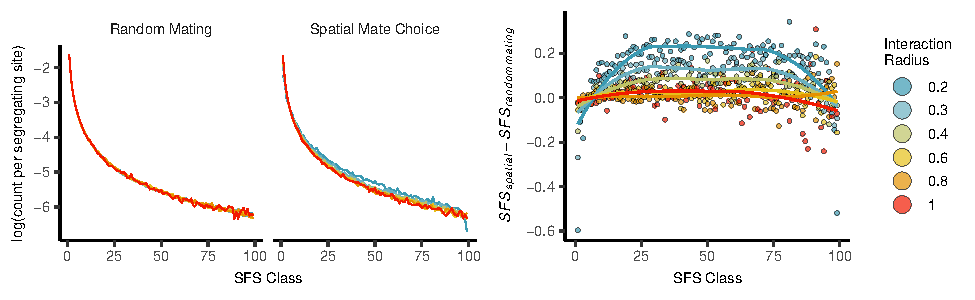
\includegraphics[width=\textwidth]{sfs_spatial_v_rm.pdf}
\caption{Scaled allele frequency distributions for random mating and spatial SLiM models under varying $\sigma$. The rightmost panel is the difference between the spatial and random-mating distributions, showing an inflation of mid-frequency sites for neighborhood sizes of less than 50. Lines are a local regression (loess) model at span 2.}
\label{fig:spectrum}
\end{figure*}

\begin{figure*}[h!]
\centering
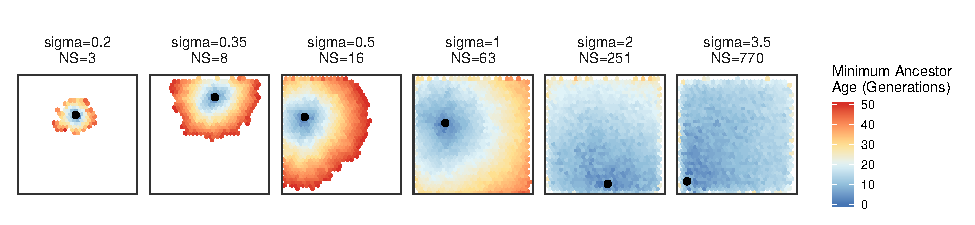
\includegraphics[width=\textwidth]{min_ancestor_age_maps.pdf}
\caption{Geographic spread of genealogical ancestors from a random individual over 50 generations, by Neighborhood size and $\sigma$. Colors are scaled by the age of the most recent ancestor.}
\label{fig:spectrum}
\end{figure*}

\begin{figure*}[h!]
\centering
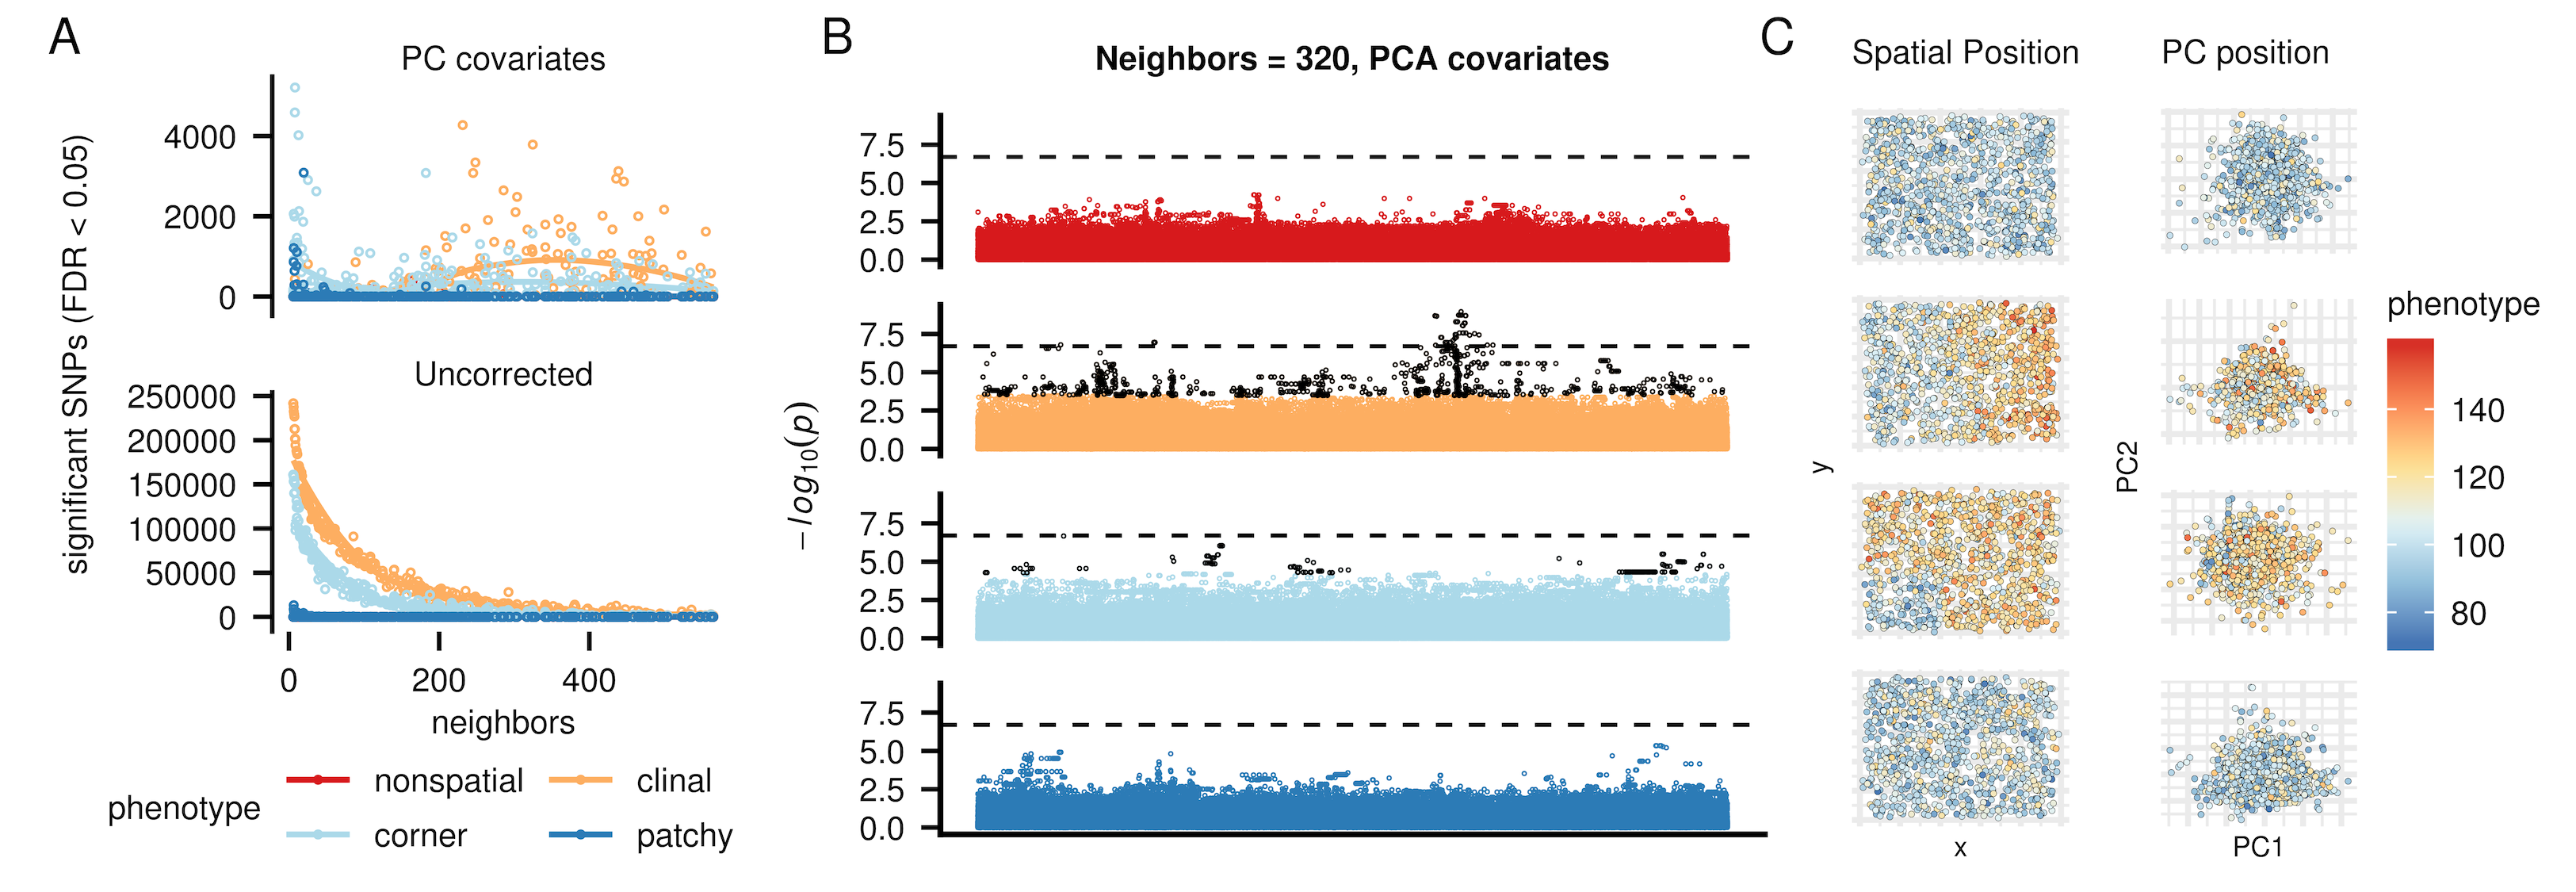
\includegraphics[width=\textwidth]{gwas_summary_sigma225.png}
\caption{Impacts of spatially correlated phenotypes and isolation by distance on GWAS. Colors represent different phenotype distributions as indicated in the figure legend. A: numbers of significant SNPs after FDR correction for linear-model GWAS conducted with (top) or without (bottom) PC covariates. B: Example Manhattan plots for a single simulation with varying phenotype distributions. Points in black are significant at an estimated FDR cutoff of 0.05, while the dotted line shows the Bonferroni-corrrected \textit{p} value of 0.05. In practice most human GWAS studies use a significance cutoff between these points. C and D show the corresponding spatial and principal component positions, colored by phenotype.}
\label{fig:spectrum}
\end{figure*}

\newpage


\bibliography{spaceness}

\end{document}



\section{Genetics Submission Guidelines}
Manuscripts submitted to \textit{GENETICS} should contain a clear description of the experimental design in sufficient detail so that the experimental analysis could be repeated by another scientist. If the level of detail necessary to explain the protocol goes beyond two paragraphs, give a short description in the main body of the paper and prepare a detailed description for supporting information.  For example, details would include indicating how many individuals were used, and if applicable how individuals or groups were combined for analysis. If working with mutants indicate how many independent mutants were isolated. If working with populations indicate how samples were collected and whether they were random with respect to the target population.


\subsection{Statistical Analysis} 

It is important to indicate what statistical analysis has been performed; not just the name of the software and options selected, but the method and model applied. In the case of many genes being examined simultaneously, or many phenotypes, a multiple comparison correction should be used to control the type I error rate, or a rationale for not applying a correction must be provided. The type of correction applied should be clearly stated. It should also be clear whether the p-values reported are raw, or after correction. Corrected p-values are often appropriate, but raw p-values should be available in the supporting materials so that others may perform their own corrections. In large scale data exploration studies (e.g. genome wide expression studies) a clear and complete description of the replication structure must be provided. 

\subsection{Data Availability}

At the end of the Materials and Methods section, include a statement on reagent and data availability. Please read the Data and Reagent Policy before writing the statement. Make sure to list the accession numbers or DOIs of any data you have placed in public repositories. List the file names and descriptions of any data you will upload as supplemental information. The statement should also include any applicable IRB numbers. You may include specifications for how to properly acknowledge or cite the data.

For example: Strains are available upon request. File S1 contains detailed descriptions of all supplemental files. File S2 contains SNP ID numbers and locations. File S3 contains genotypes for each individual. Sequence data are available at GenBank and the accession numbers are listed in File S3. Gene expression data are available at GEO with the accession number: GDS1234. Code used to generate the simulated data is provided in file S4. 


\section{Results and Discussion}

The results and discussion should not be repetitive. The results section should give a factual presentation of the data and all tables and figures should be referenced; the discussion should not summarize the results but provide an interpretation of the results, and should clearly delineate between the findings of the particular study and the possible impact of those findings in a larger context. Authors are encouraged to cite recent work relevant to their interpretations. Present and discuss results only once, not in both the Results and Discussion sections. It is sometimes acceptable to combine results and discussion. The text should be as succinct as possible. Heed Strunk and White's dictum: "Omit needless words!"

\section{Additional guidelines}

\subsection{Numbers} In the text, write out numbers nine or less except as part of a date, a fraction or decimal, a percentage, or a unit of measurement. Use Arabic numbers for those larger than nine, except as the first word of a sentence; however, try to avoid starting a sentence with such a number.

\subsection{Units} Use abbreviations of the customary units of measurement only when they are preceded by a number: "3 min" but "several minutes". Write "percent" as one word, except when used with a number: "several percent" but "75\%." To indicate temperature in centigrade, use ° (for example, 37°); include a letter after the degree symbol only when some other scale is intended (for example, 45°K).

\subsection{Nomenclature and Italicization} Italicize names of organisms even when  when the species is not indicated.  Italicize the first three letters of the names of restriction enzyme cleavage sites, as in HindIII. Write the names of strains in roman except when incorporating specific genotypic designations. Italicize genotype names and symbols, including all components of alleles, but not when the name of a gene is the same as the name of an enzyme. Do not use "+" to indicate wild type. Carefully distinguish between genotype (italicized) and phenotype (not italicized) in both the writing and the symbolism.

\subsection{Cross References}
Use the \verb|\nameref| command with the \verb|\label| command to insert cross-references to section headings. For example, a \verb|\label| has been defined in the section \nameref{sec:materials:methods}.

\section{In-text Citations}

Add citations using the \verb|\citep{}| command, for example \citep{neher2013genealogies} or for multiple citations, \citep{neher2013genealogies, rodelsperger2014characterization,Falush16}

\section{Examples of Article Components}
\label{sec:examples}

The sections below show examples of different header levels, which you can use in the primary sections of the manuscript (Results, Discussion, etc.) to organize your content.

\section{First level section header}

Use this level to group two or more closely related headings in a long article.

\subsection{Second level section header}

Second level section text.

\subsubsection{Third level section header:}

Third level section text. These headings may be numbered, but only when the numbers must be cited in the text. 

\section{Figures and Tables}

Figures and Tables should be labelled and referenced in the standard way using the \verb|\label{}| and \verb|\ref{}| commands.

\subsection{Sample Figure}

Figure \ref{fig:spectrum} shows an example figure.

\begin{figure}[htbp!]
\centering
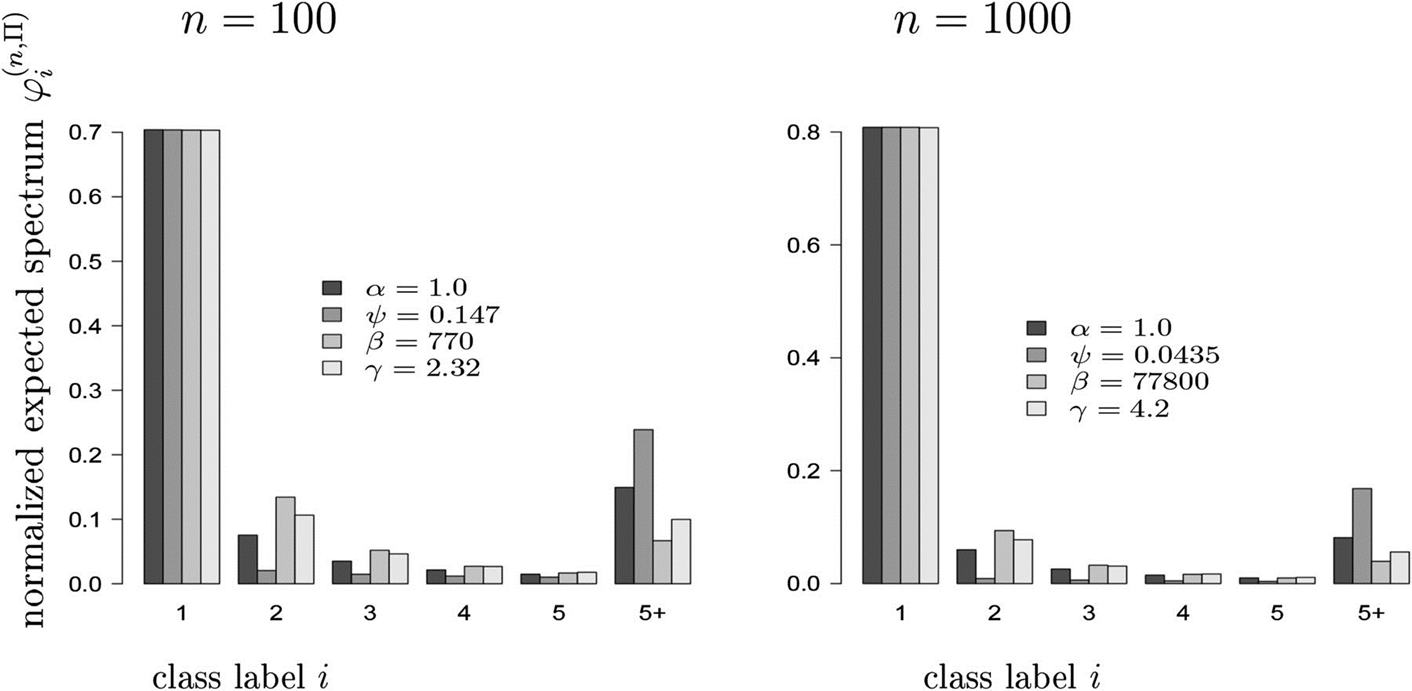
\includegraphics[width=\linewidth]{example-figure}
\caption{Example figure from \url{10.1534/genetics.114.173807}. Please include your figures in the manuscript for the review process. You can upload figures to Overleaf via the Project menu. Upon acceptance, we'll ask for your figure files to be uploaded in any of the following formats: TIFF (.tiff), JPEG (.jpg), Microsoft PowerPoint (.ppt), EPS (.eps), or Adobe Illustrator (.ai).  Images should be a minimum of 300 dpi in resolution and 500 dpi minimum if line art images.  RGB, CMYK, and Grayscale are all acceptable. Halftones should be high contrast with sharp detail, because some loss of detail and contrast is inevitable in the production process. Figures should be 10-20 cm in width and 1-25 cm in height. Graph axes must be exactly perpendicular and all lines of equal density.
Label multiple figure parts with A, B, etc. in bolded type, and use Arrows and numbers to draw attention to areas you want to highlight. Legends should start with a brief title and should be a self-contained description of the content of the figure that provides enough detail to fully understand the data presented. All conventional symbols used to indicate figure data points are available for typesetting; unconventional symbols should not be used. Italicize all mathematical variables (both in the figure legend and figure) , genotypes, and additional symbols that are normally italicized.  
}%
\label{fig:spectrum}
\end{figure}

\subsection{Sample Video}

Figure \ref{video:spectrum} shows how to include a video in your manuscript.

\begin{figure}[htbp]
\centering
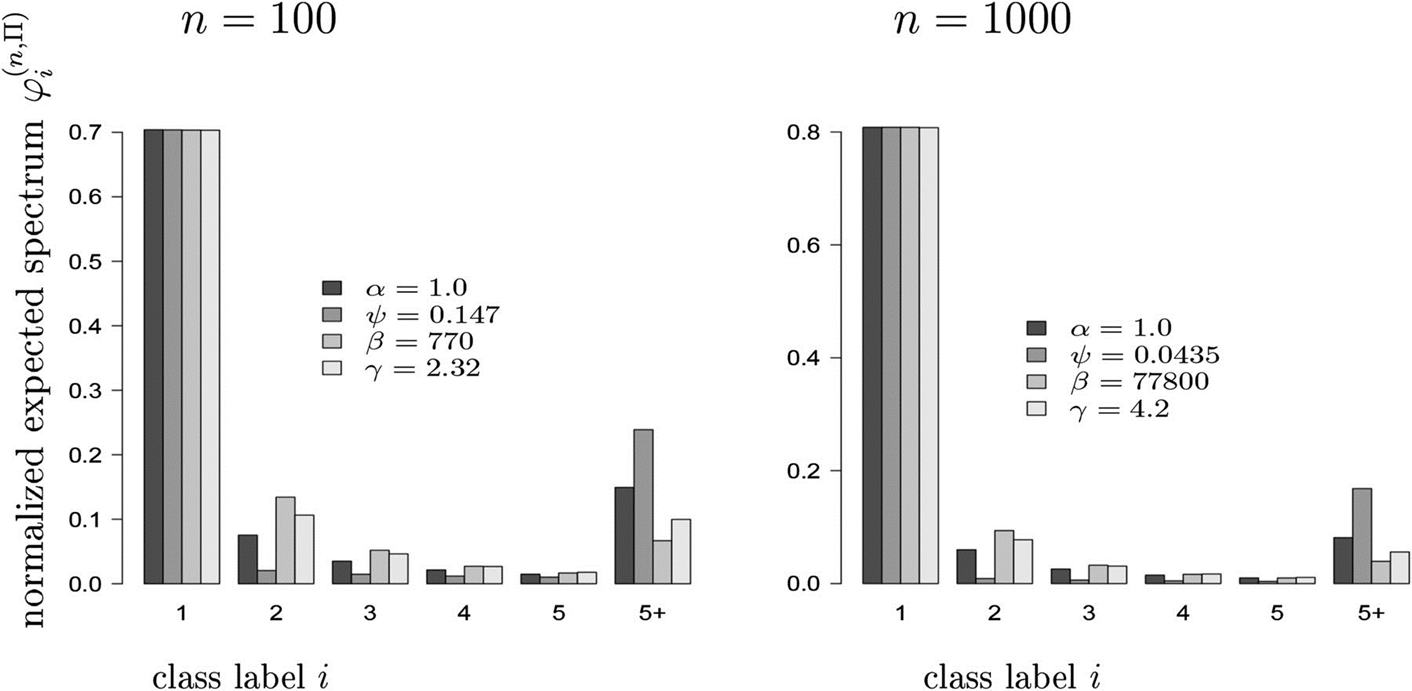
\includegraphics[width=\linewidth]{example-figure}
\caption{Example movie (the figure file above is used as a placeholder for this example). \textit{GENETICS} supports video and movie files that can be linked from any portion of the article - including the abstract. Acceptable formats include .asf, avi, .wav, and all types of Windows Media files.   
}%
\label{video:spectrum}
\end{figure}


\subsection{Sample Table}

Table \ref{tab:shape-functions} shows an example table. Avoid shading, color type, line drawings, graphics, or other illustrations within tables. Use tables for data only; present drawings, graphics, and illustrations as separate figures. Histograms should not be used to present data that can be captured easily in text or small tables, as they take up much more space.  

Tables numbers are given in Arabic numerals. Tables should not be numbered 1A, 1B, etc., but if necessary, interior parts of the table can be labeled A, B, etc. for easy reference in the text.  


\begin{table*}[htbp]
\centering
\caption{\bf Students and their grades}
\begin{tableminipage}{\textwidth}
\begin{tabularx}{\textwidth}{XXXX}
\hline
Student & Grade\footnote{This is an example of a footnote in a table. Lowercase, superscript italic letters (a, b, c, etc.) are used by default. You can also use *, **, and *** to indicate conventional levels of statistical significance, explained below the table.} & Rank & Notes \\
\hline
Alice & 82\% & 1 & Performed very well.\\
Bob & 65\% & 3 & Not up to his usual standard.\\
Charlie & 73\% & 2 & A good attempt.\\
\hline
\end{tabularx}
  \label{tab:shape-functions}
\end{tableminipage}
\end{table*}

\section{Sample Equation}

Let $X_1, X_2, \ldots, X_n$ be a sequence of independent and identically distributed random variables with $\text{E}[X_i] = \mu$ and $\text{Var}[X_i] = \sigma^2 < \infty$, and let
\begin{equation}
S_n = \frac{X_1 + X_2 + \cdots + X_n}{n}
      = \frac{1}{n}\sum_{i}^{n} X_i
\label{eq:refname1}
\end{equation}
denote their mean. Then as $n$ approaches infinity, the random variables $\sqrt{n}(S_n - \mu)$ converge in distribution to a normal $\mathcal{N}(0, \sigma^2)$.